\chapter{Chi tiết Ontology Web Language}
\paragraph{Giới thiệu }Như đã được đề cập trong phần cuối của chương trước, chức năng chính của OWL là một ngôn ngữ ontology cung cấp ngữ nghĩa cho Semantic Web. Trong nội dung chương này, chúng em sẽ giới thiệu về cú pháp, định dạng và chi tiết các thuộc tính của ngôn ngữ Ontology Web. Phiên bản Ontology Web Language chúng em sử dụng là phiên bản 2 \cite{owl2} được tổ chức W3C khuyến khích sử dụng so với phiên bản OWL cũ 1.1 . Một cách ngắn gọn OWL là một ngôn ngữ ontology dựa trên Description Logic (DL) $SROIQ_{(D)}$ \cite{DL}, với ưu điểm là khả năng mô hình hóa các đối tượng trong các lĩnh vực (domain) tri thức được biết đến thành những khái niệm (concept) và đồng thời là khả năng biểu diễn ngữ nghĩa mạnh mẽ, giúp việc suy luận có thể được thực hiện tự động thông qua các ẩn ý (implications).
\clearpage
\section{Khái quát về OWL 2}
\subsection{Tổng quan}
\begin{figure}[ht!]
	\centering
	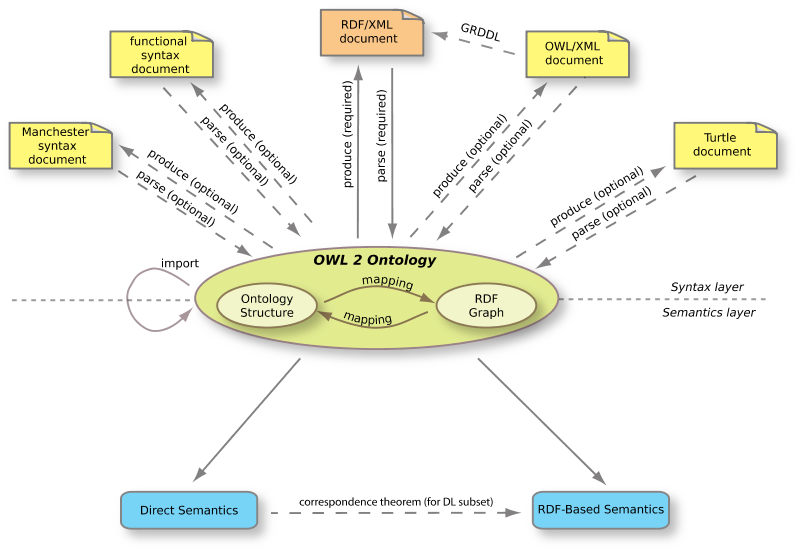
\includegraphics[width=120mm]{Figures/owl2structure.png}
	\caption{Cấu trúc của OWL 2\label{overflow}}
\end{figure}
Hình trên cho chúng ta cái nhìn tổng quan về các định dạng file, các loại cú pháp và các khả năng serialization thành RDF Graph của Ontology. Như chúng ta thấy trong hình thì hình eclipse ở giữa thể hiện khái niệm trừu tượng của một ontology, có thể hiểu là một cấu trúc trừu tượng hay một đồ thi RDF. Chúng ta có thể dùng nhiều cú pháp để biểu diễn ontology và định dạng chúng dưới dạng file khác nhau (Syntex layer trong hình), các định dạng và cú pháp này hoàn toàn có thể chuyển đổi qua lại với nhau. Lớp ngữ nghĩa trong hình (semantic layer) cho thấy ngữ nghĩa được quy định theo 2 tiêu chuẩn kỹ thuật khác nhau là Direct Semantics và RDF-Based Semantics.
\\
Phần lớn những người phát triển Ontology bằng OWL2 sẽ chỉ cần 1 cú pháp (tương đương với 1 định dạng file) và một dạng biểu diễn ngữ nghĩa.
\subsection{Ontologies}
Bất kì ontology OWL2 nào đều có thể được định dạng như một đồ thị RDF. Mối quan hệ giữa 2 cách này được quy định bởi các tài liệu Mapping to RDF Graphs document [\href{http://www.w3.org/TR/owl2-overview/#ref-owl-2-rdf-mapping}{OWL 2 RDF Mapping}] \cite{mapping_rdf_graph}, trong tài liệu này định nghĩa rất rõ ràng một bảng map từ định dạng cấu trúc của ontology qua đồ thị RDF, và ngược lại. 
\subsection{Cú pháp}
Trong thực tế, một cú pháp cụ thể rất cần thiết để lưu trữ các OWL2 Ontologies và để trao đổi chúng giữa các công cụ và ứng dụng khác nhau. Cú pháp đầu tiên có khả năng hoán đổi là RDF/XML [\href{http://www.w3.org/TR/owl2-overview/#ref-rdf-syntax}{RDF Syntax}] \cite{rdfxml}. Ngoài RDF/XML có khả năng cung cấp khả năng tương tác giữ nhiều ứng dụng OWl2 khác nhau, các loại cú pháp khác đều có thể được sử dụng. Dưới đây là bảng so sánh và liệt kê các cú pháp.
\begin{table}[H]
\begin{tabular}{ |p{3cm}|p{4cm}|p{2cm}|p{4cm}|}
\hline
Tên cú pháp & Mô tả & Trạng thái & Mục đích sử dụng\\
\hline
RDF/XML & Mapping to RDF Graphs \cite{mapping_rdf_graph} \cite{rdfxml} & Bắt buộc & Hoán đổi được ( có thể viết và đọc được bằng nhiều phần mềm OWL2)
\\
\hline
OWL/XML & XML Serialization \cite{owlxml} & Tùy chọn & Xử lý dễ dàng hơn bằng công cụ XML.
\\
\hline
Functional Syntax & Structural Specification \cite{func_syntax} & Tùy chọn & Dễ đọc và hiểu được.
\\
\hline
Manchester Syntax & Manchester Syntax \cite{man_syntax} & Tùy chọn & Có ưu thế hơn để đọc/ghi DL Ontologies
\\
\hline
Turtle & Mapping to RDF Graphs \cite{mapping_rdf_graph} & Tùy chọn, không được công nhận chính thức & Có ưu thế để đọc/ghi RDF triples
\\
\hline
\end{tabular}
\caption{Bảng so sánh các cú pháp của OWL2\label{overflow}}
\end{table}
\subsection{Một số ví dụ của các syntax}

\subsubsection{Functional Syntax}
\begin{verbatim}
// Khai báo lớp
Declaration (Class (Animal)) 
Declaration (Class (Grass))) 
// Khai báo Object Property
Declaration (ObjectProperty (canEat))  
// Khai báo sub Class expression
SubClassOf (Cow Animal)  
// Khai báo sub Class Expression
SubClassOf (Cow ObjectSomeValueFrom(canEat Grass))  
\end{verbatim}

\subsubsection{RDF/XML Syntax}
\begin{verbatim}
T(Animal) rdf:type owl:Class
T(Grass) rdf:type owl:Class
T(canEat) rdf:type owl:ObjectProperty
T(Cow) rdfs:subClassOf T(Animal) 
T(Cow) rdfs:subClassOf T(_:x owl:someValuesFrom T(Grass))
\end{verbatim}


\subsubsection{OWL/XML Syntax}
\begin{verbatim}
<Declaration>
       <Class IRI="#Animal"/> // Khai báo lớp Animal
</Declaration>
<Declaration>
       <Class IRI="#Grass"/> // Khai báo lớp Grass
</Declaration>
<Declaration>
       <ObjectProperty IRI="#canEat"/> // Khai báo Object Property 
</Declaration>
<SubClassOf>
       <Class IRI="#Cow"/>
       <Class IRI="#Animal"/>  // Khai báo sub Class expression
</SubClassOf>
<SubClassOf>
       <Class IRI="#Cow"/>
<ObjectAllValuesFrom>
<ObjectProperty IRI="#canEat"/>  // Khai báo sub Class expression
       <Class IRI="#Grass"/>
</ObjectAllValuesFrom>
</SubClassOf>
\end{verbatim}


\subsubsection{Manchester Syntax}

\begin{verbatim}
Class: Cow 
    SubClassOf: Animal 
    SubClassOf: canEat some Grass
Class: Grass
ObjectProperty: canEat
\end{verbatim}


\section{Các thuộc tính chi tiết của OWL2}
Ngôn ngữ Ontology Web Language 2 (hay OWL 2) đảm nhiệm chức năng thể hiện ngữ nghĩa cho Semantic Web như chúng ta đã thấy trong hình Semantic Web Stack. OWL2 ontologies cung cấp các lớp (class), đặc tính (property), cá thể (individual) và các giá trị dữ liệu (data value), tất cả chúng sẽ được biểu diễn bằng các tài liệu và cú pháp được đề cập ở trên, phần này sẽ đi vào giải thích các thành phần vừa nêu ra của một ontology được viết bằng ngôn ngữ OWL2 . Đây cũng chính là các thành phần cấu trúc mà thư viện OWLAPI \cite{owlapi} áp dụng để xây dựng nên bộ thư viện giúp người phát triển ứng dụng ontology tương tác dễ dàng hơn với các tài liệu ontology.
Đầu tiên chúng em xin được giới thiệu tới đối tượng lớn nhất trong quy định của ngôn ngữ OWL2. 
\\
Tiếp theo, chúng em xin được trình bày về một qua các định nghĩa những thành phần cấu tạo của ontology mà có ảnh hướng đến quá trình xây dựng ứng dụng, các thành phần không liên quan sẽ không được đề cập.
\section{Định nghĩa các thành phần cấu tạo nên một ontology}
\subsection{Ontology IRI và Version IRI}
Mỗi ontology đều có thế có\textit{một ontology IRI} \cite{iri} \textsuperscript{*} (Internationalized Resource Identifier), dùng để định danh cho ontology. Nếu một ontology có một ontology IRI, thì ontology này có thể có thêm một version IRI, dùng để xác định phiên bản cho ontology này. Version IRI có thể trùng hoặc không cần thiết phải trùng với ontology IRI. Một ontology không có ontology IRI thì không có version IRI.
Dưới đây là những quy ước chọn ontology IRIs và version IRIs trong OWL2. Những đặc điểm kỹ thuật này không cung cấp cơ chế nào để làm chúng phải được tuân theo trên toàn hệ thống web. Tuy nghiên, những công cụ hay ứng dụng OWl2 \textit{nên} sử dụng những quy ước này để dễ dàng tìm ra lỗi trong những ontology mà chúng xử lý.
{\let\thefootnote\relax\footnotetext{*\textit{
			Internationalized Resource Identifier: giao thức bổ sung cho Uniform Resource Universal Character Set (Unicode/ISO 10646).}}
}
\begin{itemize}
\item Nếu một ontology có một ontology IRI nhưng không có version IRI, thì \textit{không nên tồn tại} một ontology với trùng ontology IRI vừa đặt.
\item Nếu một ontology có một ontology IRI và một version IRI, thì \textit{không nên tồn tai} một ontology khác với trùng ontology IRI và version IRI vừa đặt.
\item Tất cả các cách kết hợp khác của ontology IRI và version IRI không cần đòi hỏi tính duy nhất (unique). Như vậy 2 ontologies khác nhau có thể không có ontology IRI và version IRI; tương tự, một ontology chưa một ontology IRI có thể cùng tồn tại cùng với một ontology khác có cùng ontology IRI vừa đặt \textbf{và} các version IRI của các ontologies này \textbf{phải} khác nhau.
\end{itemize}
Ontology IRI và các version IRI kết hợp với nhau giúp định danh một phiên bản cụ thể của của ontology từ một bộ chưa tất cả các phiên bản của một ontology cụ thể nào đó được định danh chung bằng ontology IRI. Trong mỗi bộ ontology như vậy, sẽ có chính xác một ontology được dùng nhưng một ontology hiện hành - khi dùng ontology IRI để truy vấn ontology mà không đề cập version IRI mặc định ontology co verison IRI hiện hành sẽ được trả về.

%\subsubsection{Tài liệu Ontology}
%Bản chất OWL 2 Ontology chỉ là một khái niệm trừu tượng chiếu theo định nghĩa trong các thuộc tính cấu tạo của nó, để biểu diễn những ngữ nghĩa trong ontology và lưu trữ chúng, chúng ta cần một dạng tài liệu được quy ước. Cụm từ "Tài liệu ontology" (\textit{Ontology Document}) muốn nói đến khả năng một số lượng lớn ontologies có thể được lưu giữ trong một tài liệu thực sự được biểu diễn dưới dạng một trong các cú pháp vừa nếu ở phần. 

\subsection{Thực thể, trực nghĩa và cá thể ẩn danh - Entities, Literals and Anonymous Individuals}
Các thực thể (entities) là thành phần cơ bản nhất của OWL2 Ontology, chúng định nghĩa các từ vừng - cụ thể là những đặt tên ra các khái niệm (named term) - của một ontology. Bên cạnh các thực thể, OWL 2 ontologies thường có thêm các trực nghĩa (literals), như strings hay integers.
\begin{figure}[ht!]
	\centering
	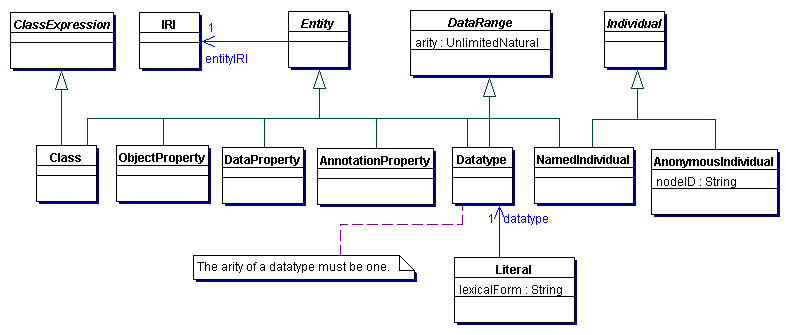
\includegraphics[width=150mm, height=80mm]{Figures/entities.png}
	\caption{Entities, Literals, Anonymous Individuals trong OWL2 \label{overflow}}
\end{figure}
\\
Cấu trúc của các thực thể và trực nghĩa trong OWL 2 được thể hiện trong hình bên. Các lớp (classes), kiểu dữ liệu (datatypes), thuộc tính đối tượng (object properties), thuộc tính dữ liệu (data properties), thuộc tính chú thích và các cá thể có tên đều được gọi chung là các thực thể (entities), tất cả chúng được được định danh bằng một IRI duy nhất. 
\begin{itemize}
\item Lớp (class) đại diện cho một tập gồm nhiều cá thể(individuals).
\item Kiểu dữ liệu (datatype) là một tập của các trực nghĩa như strings hoặc integers.
\item Thuộc tính đối tượng và dữ liệu (object \& data property) được sử dụng để biểu diễn các mối quan hệ giữa các cá thể với cá thể khác và giữa cá thể với trực nghĩa (literal) trong một lĩnh vực (domain) nào đó.
\item Thuộc tính chú thích (annotation) được dùng để đưa thêm những thông tin không có tính ngữ nghĩa( non-logical) như các chú thích, giải nghĩa, ngôn ngữ gắn với ontologies, các phát biểu/ tiên đề (axioms) và các thực thể.
\item  Các cá thể có tên có thể được dụng để biểu diễn một đối tượng cụ thể từ một lớp nào đó.
\end{itemize}
Bên cạnh các cá thể có tên, OWL2 còn cung cấp một khái niệm gọi là các cá thể ẩn danh (anonymous individuals) - là cá thể tương tự với các node trống (blank nodes) trong RDF Concept \cite{rdf_concept} và được truy xuất ngay bên trong ontology mà chúng được sử dụng. Cuối cùng, OWL 2 cung cấp thêm cho cac trực nghĩa (literals), một dạng dữ liệu string gọi là định dạng nghĩa bằng từ ngữ (lexical form) và một dạng dữ liệu để chỉ dẫn cách ontology có thể hiểu chuỗi này.
% Classes 
\subsubsection{Lớp (Classes)}
Lớp được hiểu như tập hợp các cá thể. Hai lớp với IRIs \textit{owl:Nothing} và \textit{owl:Thing} là các lớp được định nghĩa sẵn trong OWL2 với ý nghĩa như sau:
\begin{itemize}
\item \textbf{owl:Thing} là tập hợp gồm tất cả các cá thể.
\item \textbf{owl:Nothing} là tập hợp rỗng.
\end{itemize}
Không nên sử dụng 2 định nghĩa trên để gán cho bất kì lớp nào trong OWL 2 DL Ontology. Ví dụ:
\begin{verbatim}
SubClassOf( a:Child a:Person) 
\end{verbatim}
\textbf{Giải thích:} Mỗi đứa trẻ đều là một người.

% Datatypes
\subsubsection{Kiểu dữ liệu (datatypes)}
Kiểu dữ liệu là thực thể được xem như tập hợp của các giá trị dữ liệu. Như vậy, kiểu dữ lữ liệu cũng tương tự lớp, khác biệt chính là thay vì chứa các cá thể (individuals) như lớp thì lại chứ các giá trị dữ liệu như strings, numbers, Kiểu dữ liệu có thể được dùng tạo ra các dữ liệu giới hạn (datarange). Ví dụ kiểu dữ liệu \textit{xsd:positiveInteger} đại diện cho tập hợp gồm tất cả các số nguyên dương. Nó được sử dụng để quy định kiểu dữ liệu mà thuộc tính \textit{hasAge} có thể chấp nhận:

\begin{verbatim}
DataPropertyRange( a:hasAge xsd:positiveInteger) 
\end{verbatim}

\textbf{Giải thích:} thuộc tính dữ liệu a:hasAge chỉ được phép là các số nguyên dương.

% Object Properties
\subsubsection{Thuộc tính đối tượng (object properties)} 
Thuộc tính đối tượng kết nối các cặp cá thể - tạo ra mối liên hệ (relationship) giữa các cá thể. Tương tự lớp cũng có 2 thuộc tính đối tượng được định nghĩa sẵn trong OWL 2 với ý nghĩa như sau:
\begin{itemize}
\item \textbf{owl:topObjectProperty} kết nối tất cả các cặp cá thể có thể kết nối.
\item \textbf{owl:bottomObjectProperty} không kết nối bất kì cặp cá thể nào. 
\end{itemize}
Tương tự lớp cũng không nên sử dụng 2 định nghĩa trên để gán cho bất kỳ thuộc tính đối tượng nào trong OWL 2 DL Ontology. Ví dụ:
\begin{verbatim}
ObjectPropertyAssertion( a:parentOf a:Peter a:Chris)  
\end{verbatim}
\textbf{Giải thích:} Peter là ba mẹ của Chris. Thuộc tính đối tượng \textit{a:parentOf} được dùng để nói lên mối quan hệ giữ các cá thể trong ví dụ trên.

% Data Properties
\subsubsection{Thuộc tính dữ liệu (data properties)}
Thuộc tính dữ liệu liên kết các cá thể với các trực nghĩa. Trong một vài hệ thống biểu diễn tri thức, thuộc tính dữ liệu chức năng được gọi là thuộc tính.
Hai định nghĩa sẵn \textit{owl:topDataProperty} và \textit{owl:bottomDataProperty} có ý nghĩa như sau
\begin{itemize}
\item \textbf{owl:topDataProperty} liên kết tất cả cá thể với tất cả các trực nghĩa.
\item \textbf{owl:bottomDataProperty} không liên kết bất kì cá thể với trực nghĩa nào.
\end{itemize}
Tương tự lớp và thuộc tính đối tượng, 2 phát biểu \textit{top} và \textit{bottom} trên cũng không nên được sử dụng để gán cho bất kì thuộc tính dữ liệu nào. Mỗi thuộc tính dữ liệu \textit{a:hasName} chứa tên đầy đủ của mỗi người. Ví dụ nó có thể được sử dụng như trong phát biểu sau:

\begin{verbatim}
DataPropertyAssertion( a:hasName a:Steve "Steve Job") 
\end{verbatim}

\textbf{Giải thích:} Tên của Steve là "Steve Job".

% Individuals
\subsubsection{Cá thể (Individuals)}
Cá thể trong OWL2 là một đối tượng cụ thể thuộc một tập/lớp (domain/class). Có 2 dạng cá thể trong cú pháp OWL2. \textit{Cá thể có tên} được khai báo tên một cách rõ ràng để có thể sử dụng trong bất kì ontology nào bằng cách truy vấn tới IRI có chứa tên của nó. Ngược lại, cá thể ẩn danh (Anonymous Individuals) không có tên gọi toàn cục và chỉ truy vấn được trong nội bộ của ontology chứa chúng.

% Named Individuals
\paragraph{Cá thể có tên (Named Individuals)} được định danh bằng một IRI. Vì vậy, nên cá thể có tên cũng là một thực thể (entity) tương tự lớp, thuộc tính và kiểu dữ liệu. Ví dụ khai báo một các thể thuộc 1 lớp:


\begin{verbatim}
ClassAssertion( a:Person a:Peter)
\end{verbatim}


\textbf{Giải thích:} Peter là một người.

% Anonymous Individuals
\paragraph{Cá thể ẩn danh (Anonymous Individuals)} Nếu cần một cá thể chỉ sử dụng ở nội bộ ontology, chúng ta có thể sử dụng cá thể ẩn danh, được định danh bằng một node ID cục bộ thay vì sử dụng IRI toàn cục. Cá thể ẩn danh tương tự như một node rỗng trong đồ thị RDF \cite{rdf_concept}. Ví dụ khai báo thuộc tính đối tượng giữa cá thể ẩn danh với cá thể có tên:

\begin{verbatim}
ObjectPropertyAssertion( a:liveAt a:Peter _:a1)
ObjectPropertyAssertion( a:city _:a1 a:HCM)
ObjectPropertyAssertion( a:district _:a1 a:ThuDuc)
\end{verbatim}

\textbf{Giải thích:} Peter sống ở một địa chỉ nào đó (chưa biết). Mà địa chỉ chưa biết này nằm trong thành phố Hồ Chí Minh và nằm trong quận Thủ Đức.

% Literals
\subsubsection{Trực nghĩa (Literals)}
Trực nghĩa biểu diễn các giá trị dữ liệu như chuỗi và số nguyên. Mỗi trực nghĩa gồm một chuỗi định dạng được định nghĩa bới người dùng (lexical form), và một kiểu dữ liệu được hỗ trợ bởi OWL2 \cite{owl2spec} . Một trực nghĩa gồm một chuỗi định dạng \textit{"abc"} và một kiểu dữ liệu (Datatype) định danh bởi IRI \textit{datatypeIRI} được định nghĩa như sau \verb|"abc"^^datatypeIRI|. Thêm nữa, các trực nghĩa mà kiểu dữ liệu của chúng là \textit{rdf:PlainLiteral} có thể được viết tắt trong functional-syntax của OWL2 ghi lại trong tài liệu thành dạng trực nghĩa rỗng RDF \cite{rdf_concept}. Cú pháp viết tắt này chỉ đơn giản là một định dạng ngắn gọn hơn, chúng không có ảnh hưởng đến ý nghĩa của khai báo trực nghĩa. Viết tắt chủ yếu là để phục vụ cho việc parsing:
\begin{itemize}
\item Trực nghĩa dạng \verb|"abc@"^^rdf:PlainLiteral| được viết tắt thành \verb|"abc"|.
\item Trực nghĩa dạng \verb|"abc@langTag"^^rdf:PlainLiteral| trong đó \textit{"langTag"} không rỗng được viết tắt thành \verb|"abc"@langTag|.
\end{itemize}
\textbf{Cú pháp:}
\begin{verbatim}
Literal      := typedLiteral | stringLiteralNoLanguage 
| stringLiteralWithLanguage
typedLiteral := lexicalForm '^^' Datatype
lexicalForm  := quotedString
stringLiteralNoLanguage := quotedString
stringLiteralNoLanguage := quotedString
\end{verbatim}
Một số ví dụ:
\begin{verbatim}
"1"^^xsd:integer  // trực nghĩa biểu diễn số nguyên dương 1
"abc"^^xsd:string // trực nghĩa biểu diễn chuỗi "abc"
\end{verbatim}

% Entity Declarations and Typing
\subsubsection{Khai báo thực thể}
Mỗi IRI \textit{I} được sử dụng trong OWL 2 ontology \textit{O} cần được khai báo để sử dụng. Phát biểu khai báo một thực thể \textit{I} nhằm đảm bảo rằng \textit{O} phải chứa \textit{I}. Hai mục tiêu của phát biểu này:
\begin{itemize}
\item Khẳng định sự tồn tại trong \textit{I} trong \textit{O}
\item Khai báo gắn với loại của thực thể \textit{I} - phân loại xem \textit{I} có phải là một lớp, một kiểu dữ liệu, mặt thuộc tính đối tượng, một thuộc tính dữ liệu, một đặt tính chú thích hay một cá thể.
\end{itemize}
Bối cảnh sử dụng khái báo \textbf{Declaration} thường gắn liền với chức năng \textit{Add New Class/Property/Datatype} trong một Ontology Editor nào đó.
\\ \textbf{Cú pháp:}
\begin{verbatim}
Declaration := 'Declaration' '(' axiomAnnotations Entity ')'
Entity :=
'Class' '(' Class ')' |
'Datatype' '(' Datatype ')' |
'ObjectProperty' '(' ObjectProperty ')' |
'DataProperty' '(' DataProperty ')' |
'AnnotationProperty' '(' AnnotationProperty ')' |
'NamedIndividual' '(' NamedIndividual ')'
\end{verbatim}
\textbf{Ví dụ:}
\begin{verbatim}
Declaration( Class( a:Person ) )
Declaration( NamedIndividual( a:Peter ) )
\end{verbatim}

% Property Expression
\subsection{Mô tả thuộc tính (Property Expression)}
Các thuộc tính được sử dụng trong OWL 2 để tạo ra các mô tả thuộc tính.

% Object Property Expression
\subsubsection{Mô tả thuộc tính đối tượng (Object Property Expression)}
Thuộc tính đối tượng được sử dụng trong OWL 2 để tạo thành các mô tả thuộc tính đối tượng (object property expression), diễn tả các mối quan hệ giữa các cặp cá thể. Chúng được diễn giải trong tài liệu cấu trúc chi tiết của OWL 2 như trong hình sau.
\begin{figure}[h!]
	\centering
	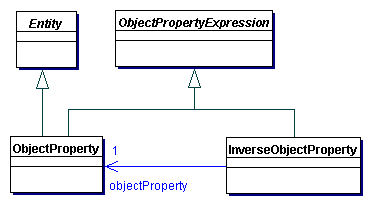
\includegraphics[width=120mm]{Figures/object_property_expression.png}
	\caption{Mô tả thuộc tính đối tượng OWL 2\label{overflow}}
\end{figure}
Như được thể hiện trong hình, OWL 2 hỗ trợ 2 loại mô tả thuộc tính đối tượng. Thuộc tính đối tượng là dạng đơn giản của mô tả thuộc tính đối tượng, thuộc tính đối tượng nghịch đảo (inverse object properties) cho phép thể hiện các mối quan hệ 2 chiều giữa biểu hiện các mô tả lớp (class expression) và các phát biểu (axiom).
\\ \textbf{Mô tả thuộc tính đối tượng nghịch đảo}

\begin{verbatim}
ObjectPropertyAssertion( a:fatherOf a:Peter a:Steve) 
// Peter là ba của Steve
\end{verbatim}}
Với phát biểu trên, ontology sẽ hiểu \textit{a:Steve} liến kết với \textit{a:Peter} qua một thuộc tính nghịch đảo của \textit{a:fatherOf} là \textit{ObjectInverseOf( a:fatherOf)}. Chúng ta cũng có thể khai báo tường minh nghịch đảo của \textit{a:fatherOf} bằng phát biểu  \textit{InverseObjectProperties( a:fatherO a:childOf )}.

% Data Property Expression
\subsubsection{Mô tả thuộc tính dữ liệu (Data Property Expression)}
Tương đương với biểu hiện thuộc tính đối tượng, trong tài liệu cấu trúc chi tiết của OWL2 cũng giới thiệu định nghĩa mô tả thuộc tính dữ liệu  (data property expressions), nhằm biểu diễn mối quan hệ giữa một cá thể và một trực nghĩa. Cấu trúc của mô tả thuộc tính dữ liệu thể hiện trong hình bên. Như chúng ta thấy thuộc tính dữ liệu (data property) cũng chính là 1 mô tả thuộc tính dữ liệu (data property expression), cấu trúc như vậy được xây dựng nhằm tạo thuận lợi cho nhu cầu mở rộng sau này nếu có.
\begin{figure}[h!]
	\centering
	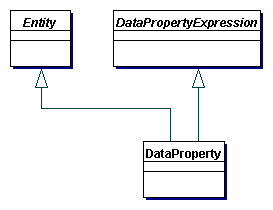
\includegraphics[width=110mm]{Figures/data_property_expression.png}
	\caption{Cấu trúc của mô tả thuộc tính dữ liệu OWL 2\label{overflow}}
\end{figure}

%Data ranges
\subsection{Miền dữ liệu (Data Range)}
Kiểu dữ liệu như\textit{xsd:string} hoặc \textit{xsd:integer} và trực nghĩa \verb|"1"^^xsd:integer| được dùng để biểu diễn miền dữ liệu - tập hợp danh sách có thứ tự (tuples) của các trực nghĩa, mà mỗi phần tử trong danh sách này chỉ chứa một trực nghĩa duy nhất để định nghĩa chính nó. Miền dữ liệu được dùng để tạo ra ràng buộc (hay những dữ liệu hợp lệ) cho thuộc tính dữ liệu. Cấu trúc của miền dữ liệu trong OWL 2 được mô tả trong hình. Thành phần đơn giản của miền dữ liệu chính là kiểu dữ liệu : một kiểu dữ liệu (Datatype) cũng chính là một miền dữ liệu (Data Range).
\begin{figure}[h!]
	\centering
	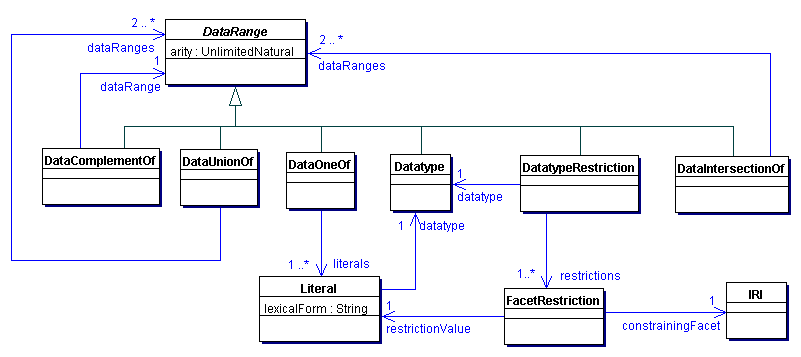
\includegraphics[width=150mm, height=80mm]{Figures/datarange.png}
	\caption{Cấu trúc miền dữ liệu (data range) quy định theo OWL 2\label{overflow}}
\end{figure}

% DataIntersectionOf
\subsubsection{Giao của các miền dữ liệu (Intersection of Data Ranges)}
Giao của miền dữ liệu \textit{DataIntersectionOf(} $DR_{1} ... DR_{n}$ \textit{)}  chứa tất cả các danh sách của các trực nghĩa nằng trong $DR_{i}$ với $1 <= i <= n$. Tất cả miền dữ liệu $DR_{i}$ phải có cùng số lượng tham số, và cũng phải có cùng số lượng số kết quả trả về. Ví dụ về miền dữ liệu chỉ chứa số 0:
\begin{verbatim}
DataIntersectionOf( xsd:nonNegativeInteger xsd:nonPositiveInteger )
\end{verbatim}

% DataUnionOf
\subsubsection{Hội của các miền dữ liệu (Union of Data Ranges)}
Điều kiện về số lượng tham số và số lượng kết quả trả về của từng $DR_{i}$ với điều kiện $1 <= i <= n$ phải giống nhau. Cú pháp \textit{DataIntersectionOf( $DR_{1} ... DR_{n}$ )}. Ví dụ về việc miền dữ liệu chứa tất cả các chuỗi và số nguyên:
\begin{verbatim}
DataUnionOf( xsd:string xsd:integer )
\end{verbatim}

% DataComplementOf
\subsubsection{Phủ định của miền dữ liệu (Complement of Data Ranges)}
Cú pháp \textit{DataComplementOf( DR )} chứa tất cả các miền dữ liệu còn lại trong năng trong miền dữ liệu \textit{DR}. Yêu câu số lượng tham số và kết quả phải bằng \textit{DR}
\begin{verbatim}
DataComplementOf( xsd:positiveInteger )
\end{verbatim}
\textbf{Giải thích:} miền dữ liệu trên chứa tất cả số nguyên âm, số 0; và chứa tất cả chuỗi (strings) vì chuỗi không phải số nguyên dương.

% DataOneOf
\subsubsection{Liệt kê trực nghĩa (Enumeration Of Literals)}
Một danh sách liệt kê các trực nghĩa (literals) với cú pháp \textit{DataOneOf(} $lt_{1} ... lt_{n}$ \textit{)},  $lt_{i}$ với $1 <= i <= n$.  Miễn dữ liệu chỉ áp dụng lên một trực nghĩa nằm trong danh sách (\textit{"oneOf"}). Ví dụ khai báo miền dữ liệu cho thuộc tính dữ liệu \textit{canMoveOnOrIn} chỉ có thể là một trong 4 giá trị chuỗi \textit{"OnRoadOrOffRoad"}, \textit{"Rail"}, \textit{"Sky"} và \textit{"Water"}.
\begin{verbatim}
DataPropertyRange(:canMoveOnOrIn 
     DataOneOf("OnRoadOrOffRoad" "Rail" "Sky" "Water"))
\end{verbatim}

% Datatype Restrictions
\subsubsection{Ràng buộc cho kiểu dữ liệu (Datatype Restrictions)}
Một ràng buộc cho kiểu dữ liệu (hay một tập các giá trị hợp lệ của kiễu dữ liệu) \textit{DatatypeRestriction(} $DT$ $F_{1}$ $lt_{1}$ ... $F_{n}$ $lt_{n}$ \textit{ )} gồm một kiểu dữ liệu đơn (unary datatype) $DT$ và $n$ cặp $($ $F_{i}$, $lt_{i}$ $)$. Vùng dữ liệu hợp lệ được tính ra bằng cách hạn chế vùng giá trị của $DT$ và lấy giao tất cả các cặp $(F_{i}$, $v_{i}$ $)$ trong đó $v_{i}$ là giá trị dữ liệu của trực nghĩa $lt_{i}$. Ví dụ miền dữ liệu sau chỉ gồm đúng các số 5,6,7,8,9:
\begin{verbatim}
DatatypeRestriction( xsd:integer 
xsd:minInclusive "5"^^xsd:integer xsd:maxExclusive "10"^^xsd:integer )
\end{verbatim}

% Class Expressions
\subsection{Mô tả lớp (Class Expression)}
Trong OWL2, các lớp và mô tả thuộc tính (property expressions) được sử dụng để xây dựng nên các mô tả lớp, hay chúng được gọi là các miêu tả hoặc trong thuật ngữ của Description Logic chúng được gọi là \textit{những khái niệm phức tạp}. Các mô tả lớp 
biểu diễn tập hợp các cá thể bằng cách chính thức đặt ra các điều kiện quy định cho các thuộc tính của các cá thể này; cá thể nào có những thuộc tính phù hợp hay thỏa những quy định đó được xem là một thành viên của mô tả lớp đang xét. Có 5 dạng mô tả lớp chính. Sau đây chúng em xin được nêu ra 3 dạng 
% Propositional Connectives and Enumeration of Individuals
\subsubsection{Các mệnh đề logic và liệt kê cá thể}
\begin{figure}[h]
	\centering
	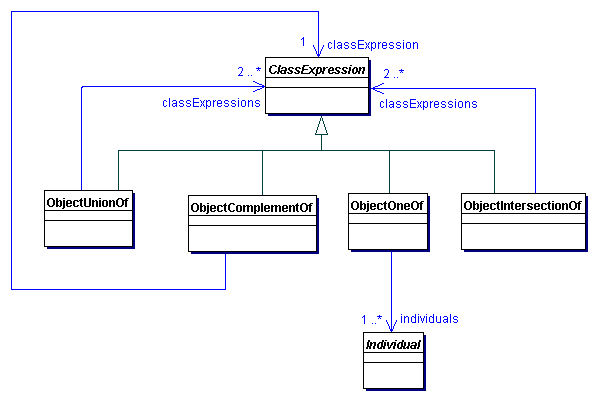
\includegraphics[width=150mm]{Figures/ce_0.png}
	\caption{Mô tả lớp với các khai báo mệnh đề trong OWL 2\label{overflow}}
\end{figure}
OWL2 cho phép liệt kê các cá thể của một lớp, khai báo các mệnh đề logic như trong hình sau. Các khai báo \textit{ObjectIntersectionOf}, \textit{ObjectUnionOf}, và \textit{ObjectComplementOf} cho phép thực hiện các phép toán luân lý (and ,or, not) lên những mô tả lớp. \textit{ObjectOneOf} quy định chính xác những cá thể cho mô tả lớp đang khai báo.

%% Intersection of Class Expressions
\paragraph{Intersection of Class Expressions} Tập giao của các mô tả lớp \textit{ObjectIntersectionOf(} $CE_{1}$ ... $CE_{n}$ \textit{)} gồm tất cả các cá thể là thành viên của tất cả các mô tả lớp $CE_{i}$ với $1<=i<=n$. Ví dụ: 
\begin{verbatim}
ClassAssertion(a:Engineer a:Peter)  // Peter là kĩ sư.
ClassAssertion(a:Teacher a:Peter) // Peter là giáo viên.
\end{verbatim}
\textbf{Giải thích: } với khai báo như trên, một hàm ý sẽ được suy ra mà không cần khai báo đó là \textit{Peter vừa là giáo viên vừa là kĩ sư} hay tương đương với phát biểu \textit{ObjectIntersectionOf( a:Engineer a:Teacher )}. 

%% Union of Class Expressions
\paragraph{Union of Class Expressions} Tập hội của lớp \textit{ObjectUnionOf(} $CE_{1}$ ... $CE_{n}$ \textit{)} chức tất cả các cá thể là thành viên của của ít nhất một mô tả lớp $CE_{i}$ với $1<=i<=n$. Ví dụ:
\begin{verbatim}
ClassAssertion( a:Man a:Peter )	 // Peter là nam
ClassAssertion( a:Woman a:Lois ) // Lois là nữ
\end{verbatim}
\textbf{Giải thích: } với khai báo như trên, một hàm ý sẽ được suy ra mà không cần khai báo đó là \textit{cả Peter và Lois đều thuộc lớp nam hoặc nữ} hay tương đương với phát biểu O\textit{bjectUnionOf( a:Man a:Woman )}.

%% Complement of Class Expressions
\paragraph{Complement of Class Expressions} Phủ định của một mô tả lớp chứa tất cả các phần tử không thuộc mô tả lớp đó. Cú pháp \textit{ObjectComplementOf(CE)}. Ví dụ:
\begin{verbatim}
DisjointClasses( a:Man a:Woman) 
// Không có cá thể nào vừa làm nam vừa là nữ
ClassAssertion( a:Woman a:Lois) 
// Lois là nữ
\end{verbatim}
\textbf{Giải thích:} Vì \textit{Lois} là nữa và không có cá thể nào vừa là nam vừa là nữ nên \textit{Lois} thuộc lớp \textit{không phải nam} tương đương với phát biểu \textit{ObjectComplementOf( a:Man )}.

\paragraph{Enumeration of Individuals} Liệt kê các cá thể \textit{ObjectOneOf(} $a_{1}$ ... $a_{n}$ \textit{)} chứa duy nhất một cá thể $a_{i}$ với $1<=i<=n$. 

% Object Property Restrictions 
\subsubsection{Ràng buộc theo thuộc tính đối tượng (Object Property Restrictions)}
\begin{figure}[h]
	\centering
	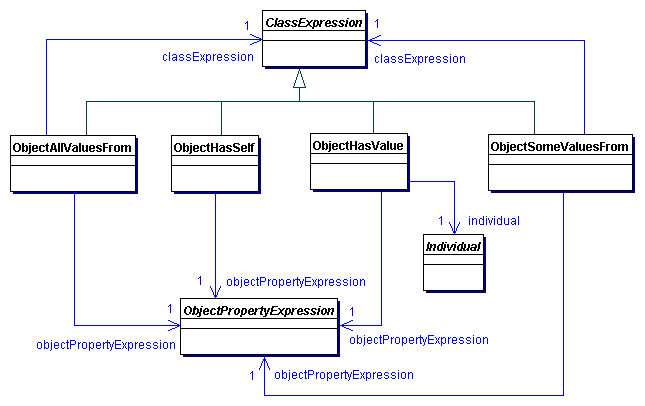
\includegraphics[width=150mm]{Figures/ce_1.png}
	\caption{Object Property Restrictions trong OWL 2\label{overflow}}
\end{figure}
Các mô tả lớp trong OWL 2 có thể được tạo ra bằng cách kết hợp chúng các thuộc tính đối tượng với bằng phát biểu như trong hình.
\paragraph{Existential Quantification} Một mô tả lớp \textit{ObjectSomeValueFrom( OPE CE )} thể hiện mối quan hệ giữa những cá thể được kết nối bởi mô tả thuộc tính đối tượng \textit{OPE} đến \textbf{ít nhất một} cá thể thuộc mô tả lớp \textit{CE}. Ví dụ:
\begin{verbatim}
ObjectPropertyAssertion( a:fatherOf a:Peter a:Steve ) 
// Peter là ba của Steve                    
ClassAssertion( a:Kid a:Steve )         
// Steve là trẻ con.
\end{verbatim} 
\textbf{Giải thích:} với khai báo như trên, một hàm ý sẽ được suy ra mà không cần khai báo đó là \textit{Peter là ba của một vài (ít nhất một) đứa trẻ} hay tương đương với phát biểu \textit{ObjectSomeValuesFrom( a:fatherOf a:Kid )}.

\paragraph{Universal Quantification} Mô tả lớp \textit{ObjectAllValuesFrom( OPE CE)} thể hiện mối quan hệ giữa những cá thể được kết nối bởi mô tả thuộc tính đối tượng $OPE$ đến \textbf{tất cả} các cá thể thuộc mô tả lớp $CE$. Ví dụ: 
\begin{verbatim}
ObjectPropertyAssertion( a:hasPet a:Peter a:Tom)
// Tom là vật nuôi của Peter
ClassAssertion( a:Cat a:Tom) 
// Tom là một con mèo
ClassAssertion( ObjectMaxCardinality( 1 a:hasPet ) a:Peter )
// Peter chỉ được phép có một vật nuôi
\end{verbatim}
\textbf{Giải thích:} với khai báo như trên, một hàm ý sẽ được suy ra mà không cần khai báo đó là \textit{Peter thuộc mô tả lớp "có tất cả vật nuôi là mèo"} hay tương đương với phát biểu \textit{ObjectAllValuesFrom( a:hasPet a:Cat )}.

\paragraph{Individual Value Restriction} Mô tả  \textit{ObjectHasValue(OPE a)} thể hiện mối quan hệ giữa tất cả các cá thể được kết nối bởi mô tả thuộc tính đối tượng \textit{OPE} và cá thể $a$. Ví dụ:
\begin{verbatim}
ObjectPropertyAssertion( a:fatherOf // Peter là ba của Steve
a:Peter a:Steve)
\end{verbatim}
\textbf{Giải thích:} với khai báo như trên, \textit{Peter thuộc mô tả lớp sau} mà không cần khai báo là \textit{ObjectHasValue( a:fatherOf a:Steve )}.

\paragraph{Self-Restriction} Mô tả \textit{ObjectHasSelf( OPE )} thể hiện mối quan hệ giữa tất cả các cá thể được kết nối bởi mô tả thuộc tính đối tượng \textit{OPE} với chính chúng. Ví dụ:
\begin{verbatim}
ObjectPropertyAssertion( a:quayQuanhTruc a:TraiDat a:TraiDat )	
// Trái đất quay quan trục của trái đất.
\end{verbatim}
\textbf{Giải thích:} với khai báo như trên, \textit{a:TraiDat thuộc mô tả lớp sau} mà không cần khai báo là \textit{ObjectHasSelf( a:quayQuanhTruc )}.

% Object Property Cardinality Restrictions
\subsubsection{Ràng buộc thuộc tính đối tượng theo số lượng}
\begin{figure}[h]
	\centering
	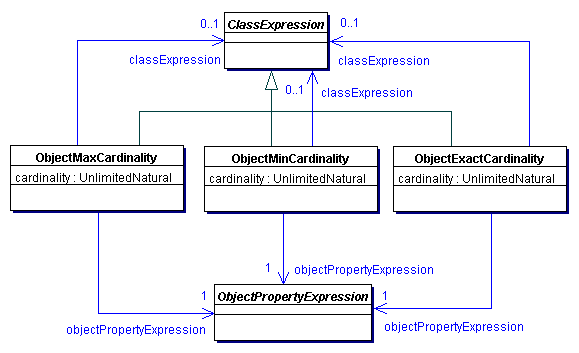
\includegraphics[width=150mm]{Figures/ce_2.png}
	\caption{Object Property Cardinality Restrictions trong OWL 2\label{overflow}}
\end{figure}
Các mô tả lớp trong OWL 2 có thể được tạo ra bằng cách đặt ra những số lượng hạn chế các cá thể mà các thuộc tính đối tượng có thể liên kết.
\paragraph{Số lượng tối thiểu (Minimum Cardinality)} - mô tả \textit{ObjectMinCardinality(n OPE  CE)} cbiểu diễn mọi các thể được kết nối bởi mô tả thuộc tính đối tượng \textit{OPE} đến số lượng tối thiểu $n$ cá thể (khác nhau) thuộc mô tả lớp \textit{CE} với $n$ là số nguyên không âm. Nếu \textit{CE} không được khai báo trong phát biểu trên mặc định sẽ là $owl:Thing$. Ví dụ:
\begin{verbatim}
ObjectPropertyAssertion( a:fatherOf 
a:Peter a:Steve )
ObjectPropertyAssertion( a:fatherOf 
a:Peter a:Bush )
ClassAssertion( a:Kid a:Steve )
ClassAssertion( a:Kid a:Bush )
\end{verbatim}
\textbf{Giải thích:} với các điều kiện như trên thì Peter sẽ được ngầm hiểu thành viên của mô tả lớp sau 
$ObjectMinCardinality($ 2 a:fatherOf a:Kid $)$ - Peter là bố của ít nhất 2 đứa trẻ.

\paragraph{Số lượng tối đa (Maximum Cardinality)} Mô tả \textit{ObjectMaxCardinality( n OPE CE)} biểu diễn mọi các thể được kết nối bởi mô tả thuộc tính đối tượng $OPE$ đến số lượng tối đa $n$ cá thể (khác nhau) thuộc mô tả lớp \textit{CE} với $n$ là số nguyên không âm. Nếu $CE$ không được khai báo trong phát biểu trên mặc định sẽ là \textit{owl:Thing}. Ví dụ:
\begin{verbatim}
ObjectPropertyAssertion( a:hasPet a:Peter a:Tom)
// Peter có vật nuôi là Tom
ClassAssertion( ObjectMaxCardinality( 1 a:hasPet ) a:Peter )
// Peter thuộc lớp "những ai có tối đa 1 vật nuôi"
\end{verbatim}
\textbf{Giải thích:} theo 2 điều kiệu trên thì Peter sẽ thuộc mô tả lớp \textit{ObjectMaxCardinality( 2 a:hasPet )} chỉ những "ai có tối đa 2 vật nuôi" (số vật nuôi <= 2), vì 2 phát biểu đầu tiên chỉ ra rằng Peter chắc chắn chỉ có một vật nuôi.

\paragraph{Số lượng chính xác (Exact Cardinality)} - mô tả \textit{ObjectExactCardinality( n OPE CE)} biểu diễn mọi các thể được kết nối bởi mô tả thuộc tính đối tượng \textit{OPE} đến số lượng chính xác $n$ cá thể (khác nhau) thuộc mô tả lớp $CE$ với $n$ là số nguyên không âm. Nếu \textit{CE} không được khai báo trong phát biểu trên mặc định sẽ là \textit{owl:Thing}. Mô tả lớp này tương được khi lấy giao của 2 mô tả số lượng tối đa và số lượng tối thiểu cùng $n$.
\begin{verbatim}
ObjectIntersectionOf( ObjectMinCardinality( n OPE CE ) 
ObjectMaxCardinality( n OPE CE ) ).
\end{verbatim}

% Data Property Restrictions
\subsubsection{Ràng buộc theo thuộc tính dữ liệu (Data Property Restrictions)}
\begin{figure}[h]
	\centering
	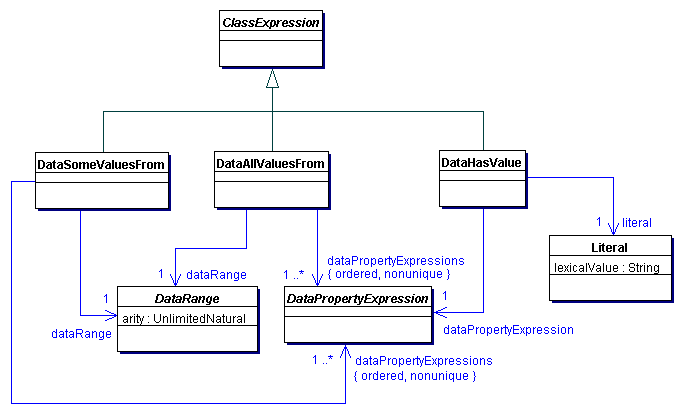
\includegraphics[width=150mm]{Figures/ce_3.png}
	\caption{Data Property Restrictions trong OWL 2\label{overflow}}
\end{figure}
Mô tả lớp dạng này được tạo ra bằng cách đặc các ràng buộc về kiểu dữ liệu, giới hạn các giá trị dữ liệu lên mô tả thuộc tính dữ liệu (data property expression) như trong hình. Những mô tả này cũng tương tự như ràng buộc thuộc tính đối tượng vừa nêu ra ở trên

%% Existential Quantification
\paragraph{Existential Quantification} Một mô tả lớp \textit{DataSomeValuesFrom(} $DPE_{1}$ ... $DPE_{n}$ $DR$ \textit{)} gồm $n$ mô tả thuộc tính dữ liệu $DPE_{i}$, $1<=i<=n$, và một miền dữ liệu (data range) $DR$ với số lượng tham số phải bằng $n$. Mô tả lớp này biểu diễn mối quan hệ dữ liệu giữa tất cả các cá thể kết nối với $DPE_{i}$ tới các trực nghĩa $lt_{i}$, $1<=i<=n$ với $($ $lt_{1}$ ... $lt_{n}$ $)$ trong $DR$. Ví dụ:
\begin{verbatim}
DataPropertyAssertion( a:hasAge a:Steve "17"^^xsd:integer ) // Steve 17 tuổi.
\end{verbatim}
\textbf{Giải thích:} Vì Steve 17 tuổi nên chúng ta ngầm hiểu rằng Steve thuộc những ai có số tuổi là số nguyên và không lớn hơn 20 tuổi, tương đương phát biểu sau
\begin{verbatim}
DataSomeValuesFrom( a:hasAge 
    DatatypeRestriction( xsd:integer xsd:maxExclusive "20"^^xsd:integer ) )
\end{verbatim}

%% Universal Quantification
\paragraph{Universal Quantification} Một mô tả lớp \textit{DataAllValuesFrom(} $DPE_{1}$ ... $DPE_{n}$ $DR$ \textit{)} gồm $n$ mô tả thuộc tính dữ liệu $DPE_{i}$, $1<=i<=n$, và một miền dữ liệu (data range) $DR$ với số lượng tham số phải bằng $n$. Mô tả lớp này biểu diễn mối quan hệ dữ liệu giữa tất cả các cá thể \textbf{chỉ} \textit{(only)} kết nối với $DPE_{i}$ tới các trực nghĩa $lt_{i}$, $1<=i<=n$ với $($ $lt_{1}$ ... $lt_{n}$ $)$ trong $DR$. Ví dụ: 
\begin{verbatim}
DataPropertyAssertion( a:hasZIP _:a1 "70000"^^xsd:integer ) 
// Mã vùng của _:a1 là số nguyên 70000
FunctionalDataProperty( a:hasZIP) 
// Mỗi đối tượng chỉ có duy nhất một mã vùng
\end{verbatim}
\textbf{Giải thích:} Mã vùng của một số quốc gia như Anh và Canada là dạng chuỗi (chứa ký tự và số), dựa vào 2 phát biểu trên chúng ta có thể hiểu rằng mã vùng của \verb|_a:1| thuộc mô tả những mã vùng \textbf{chỉ} gồm số nguyên $DataAllValuesFrom( a:hasZIP xsd:integer )$

% Literal Value Restriction
\paragraph{Ràng buộc bằng giá trị trực nghĩa - Literal Value Restriction}
Một mô tả \textit{DataHasValue(} $DPE$ $lt$ \textit{)} gồm một mô tả thuộc tính dữ liệu \textit{DPE} và một trực nghĩa $lt$, nó biểu diễn quan hệ của những cá thể nào qua \textit{DPE} tới $lt$. Ví dụ:
\begin{verbatim}
DataPropertyAssertion( a:hasAge a:Steve "17"^^xsd:integer )
\end{verbatim}
\textbf{Giải thích:} Steve là thành viên của mô tả lớp sau mà không cần khai báo "những ai 17 tuổi".
\begin{verbatim}
DataHasValue( a:hasAge "17"^^xsd:integer )
\end{verbatim}

% Data Property Cardinality Restrictions
\subsubsection{Ràng buộc thuộc tính dữ liệu theo số lượng}
\begin{figure}[h]
	\centering
	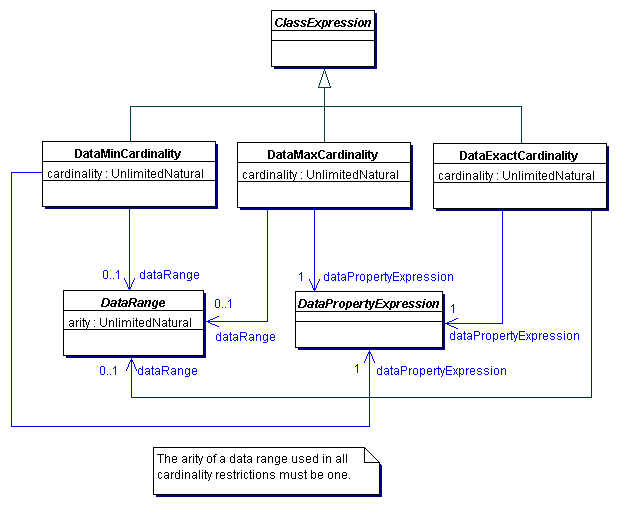
\includegraphics[width=150mm]{Figures/ce_4.png}
	\caption{Data Property Cardinality Restrictions trong OWL 2\label{overflow}}
\end{figure}
Tương tự ràng buộc thuộc tính đối tượng theo số lượng, OWL 2 cũng cho phép chúng ta tạo ra các mô tả lớp bằng cách các giá trị dữ liệu ( thay vì cá thể) mà thuộc tính dữ liệu có thể liên kết đến. Cấu trúc được mô tả như trong hình.

%% Minimum Cardinality)
\paragraph{Số lượng tối thiểu (Minimum Cardinality)} Một mô tả lớp \textit{DataMinCardinality( n DPE DR)}  biểu diễn mọi cá thể được kết nối bởi thuộc tính dữ liệu \textit{DPE} đến số lượng tối thiểu $n$ các trực nghĩa khác nhau thuộc miền dữ liệu  \textit{DR} với $n$ số nguyên không âm. Nếu \textit{DR} không được khai báo trong phát biểu trên mặc định sẽ là \textit{rdfs:Literal}. Ví dụ:
\begin{verbatim}
DataPropertyAssertion( a:hasPhoneNumber a:Steve "0123456789" )
DataPropertyAssertion( a:hasPhoneNumber a:Steve "0987654321" )
\end{verbatim}
\textbf{Giải thích:} Với 2 phát biểu như trên tồn tại, có thể hiểu Steve thuộc lớp những ai có ít nhất 2 số điện thoại \textit{DataMinCardinality(2 a:hasPhoneNumber)}.

%% Maximum Cardinality
\paragraph{Số lượng tối đa (Maximum Cardinality)} Một mô tả lớp \textit{DataMaxCardinality( n DPE DR)} biểu diễn mọi cá thể được kết nối bởi thuộc tính dữ liệu $DPE$ đến số lượng tối đa $n$ các trực nghĩa khác nhau thuộc miền dữ liệu  $DR$ với $n$ số nguyên không âm. Nếu $DR$ không được khai báo trong phát biểu trên mặc định sẽ là $rdfs:Literal$. Ví dụ:
\begin{verbatim}
DataPropertyAssertion( a:hasID a:Steve "0001" ) // Steve số CMND là 0001
FunctionalDataProperty( a:hasID ) // Mỗi người chỉ có duy nhất một số CMND
\end{verbatim}
\textbf{Giải thích:} Với 2 phát biểu như trên tồn tại, có thể hiểu Steve thuộc lớp "những ai có nhiều nhất 2 số CMND" ( số CMND <=2), \textit{DataMaxCardinality(2 a:hasID)}.

%% Exact Cardinality
\paragraph{Số lượng chính xác (Exact Cardinality)} Một mô tả lớp \textit{DataExactCardinality( n DPE DR)}  biểu diễn mọi cá thể được kết nối bởi thuộc tính dữ liệu \textit{DPE} đến số lượng chính xác $n$ các trực nghĩa khác nhau thuộc miền dữ liệu  \textit{DR} với $n$ số nguyên không âm. Nếu \textit{DR} không được khai báo trong phát biểu trên mặc định sẽ là \textit{rdfs:Literal}. Ví dụ:
\begin{verbatim}
DataPropertyAssertion( a:hasID a:Steve "0001" ) // Steve số CMND là 0001
FunctionalDataProperty( a:hasID ) // Mỗi người chỉ có duy nhất một số CMND
\end{verbatim}
\textbf{Giải thích:} Với 2 phát biểu như trên tồn tại, có thể hiểu Steve thuộc lớp "có duy nhất 1 CMND" \textit{DataExactCardinality(1 a:hasName)}.

% Axioms
\subsection{Các tiên đề (Axioms)}
{\let\thefootnote\relax\footnotetext{* Lưu ý:\textit{
			trong nội dung báo cáo này chúng em sẽ gọi vắng tắt các tiên đề - những phát biểu hiển nhiên đúng trong một lĩnh vực là \textit{những phát biểu} nhằm diễn giải các lý thuyết, nguyên lý trở dễ hiểu hơn.
		}}
}
Thành phần chính của một OWL 2 Ontology chính là một tập hợp gồm các tiên đề \textsuperscript{*} - những phát biểu mà chúng ta cho là đúng trong một lĩnh vực. OWL 2 cung cấp một loạt các loại phát biểu được mở rộng (thừa kế) từ lớp \textbf{Axiom} như trong hình. Các phát biểu có thể là các phát biểu khai báo (declarations), phát biểu về lớp, phát biểu về thuộc tính đối tượng/dữ liệu, phát biểu định nghĩa kiểu dữ liuệ, khóa (HasKey), phát biểu khẳng định (assertions), và các phát biểu để chú thích (annotations). Có thể nói những phát biểu (tiên đề) chính là những viên gạch để chúng ta xây dựng nên các tầng ngữ nghĩa (semantic) cho ontology.
\begin{figure}[!h]
	\centering
	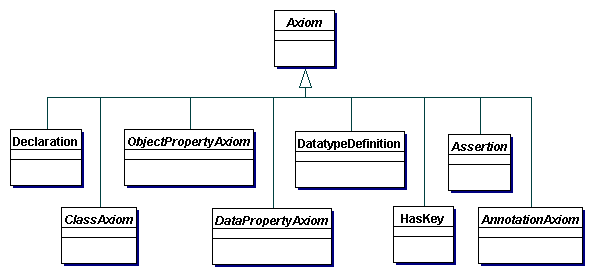
\includegraphics[width=150mm]{Figures/axioms.png}
	\caption{Các dạng phát biểu của OWL 2\label{overflow}}
\end{figure}

\subsubsection{Những phát biểu về mô tả lớp - Class Expression Axioms}
Những phát biểu này cho phép biểu diễn các loại quan hệ giữa những mô tả lớp (Class Expressions) với nhau. Có 4 phát biểu được mở rộng ra từ phát biểu này như trong hình.
\begin{figure}[!h]
	\centering
	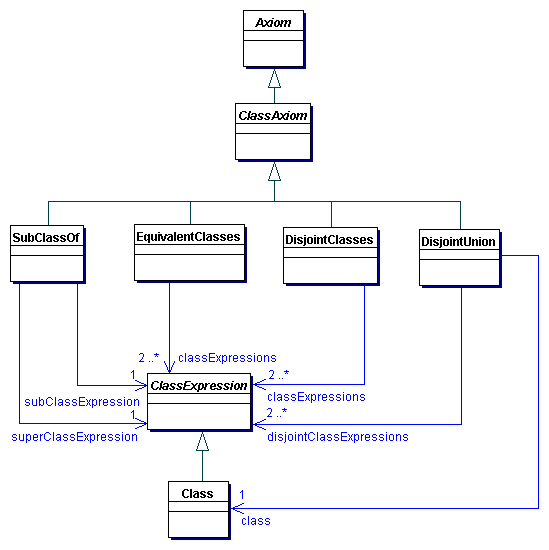
\includegraphics[width=120mm]{Figures/classAxiom.png}
	\caption{Các dạng phát biểu về lớp của OWL 2\label{overflow}}
\end{figure}

\paragraph{Phát biểu lớp con (SubClass Axioms)} - một phát biểu \textit{SubClassOf(}$CE_{1}$ $CE_{2}$ \textit{)} nói rằng mô tả lớp $CE_{1}$ là lớp con của mô tả lớp $CE_{2}$. Phát biểu này là phát biểu cơ bản trong OWL 2 được sử dụng để xây dựng một phân cấp lớp trong Ontology. Ví dụ:
\begin{verbatim}
SubClassOf( a:Driver a:Adult ) // Mỗi tài xế là một người trưởng thành.
SubClassOf( a:Adult a:Person ) // Mỗi người trưởng thành là một người.
ClassAssertion (a:Driver a:Steve ) // Steve là một tài xế.
\end{verbatim}
\textbf{Giải thích:} nhờ 2 phát biểu đầu tiên, chúng ta ngầm hiểu tài xế cũng là một người trưởng thành, cũng là một người, vì vậy tất cả những cá thể là tài xế, cũng là người trưởng thành và cũng là người -> Steve là cũng là thành viên của 2 lớp $Adult$ và $Person$.

\paragraph{Phát biểu lớp tương đương (Equivalent Classes)} - một phát biểu \textit{EquivalentClasses( $CE_{1}$ $CE_{n}$ )} nói rằng mỗi mô tả lớp $CE_{i}$, $1<=i<=n$ đều đồng nghĩa với các tất cả các mô tả lớp còn lại trong phát biểu này. Phát biểu \textit{EquivalentClasses( $CE_{2}$ $CE_{1}$ )} tương đương \textit{EquivalentClasses( $CE_{1}$ $CE_{2}$ )}. Ví dụ:
\begin{verbatim}
SubClassOf( a:Bike  a:Bicycle )
\end{verbatim}

\paragraph{Disjoint Classes} - một phát biểu \textit{DisjointClasses( $CE_{1}$ ... $CE_{n}$ )}nói rằng không cá thể nào của $CE_{i}$ thuộc $CE_{j}$ và ngược lại với $i \neq j$, $1<=i,j<=n$. Ví dụ:
\begin{verbatim}
DisjointClasses( a:Man a:Woman )	
ClassAssertion( a:Man a:Steve )
\end{verbatim}
\textbf{Giải thích:} Steve không là nữ - \textit{ObjectComplementOf( a:Girl )}, nếu chúng ta khai báo thêm $ClassAssertion($ $a:Girl$ $a:Steve)$ sẽ làm cho ontology bị thiếu tính nhất quán (sẽ được nếu rõ hơn ở các chương sau).

\subsubsection{Phát biểu về thuộc tính đối tượng (Object Property Axioms)}
Những phát biểu này cho phép biểu diễn các loại quan hệ giữa những mô tả thuộc tính đối tượng (Object Property Expressions) với nhau.
\begin{figure}[h]
	\centering
	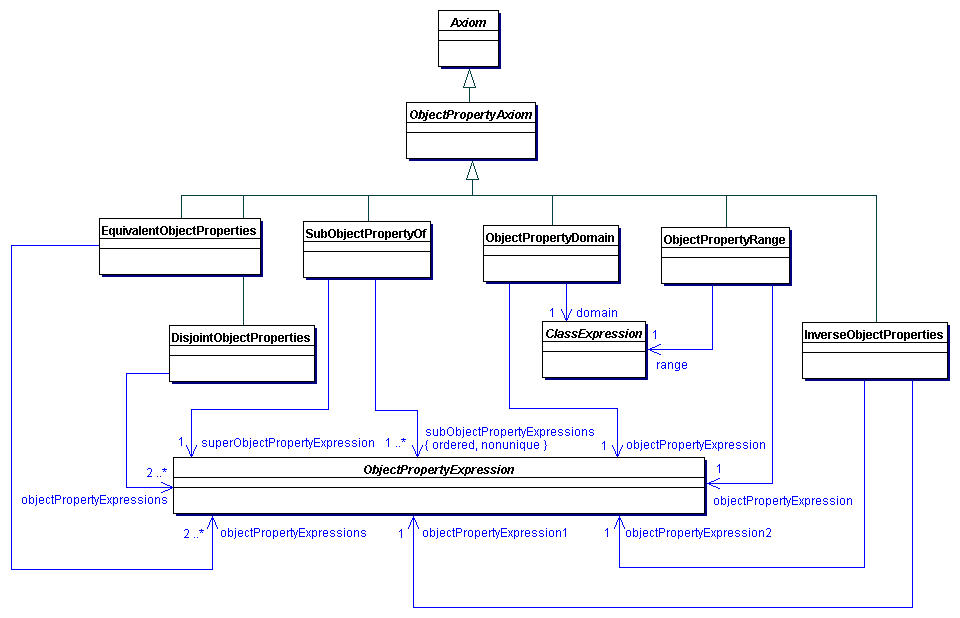
\includegraphics[width=160mm]{Figures/objectpropertyAxiom.png}
	\caption{Các dạng phát biểu về thuộc tính đối tượng của OWL 2 (phần 1)\label{overflow}}
\end{figure}

\paragraph{Thuộc tính đối tượng con (SubObjectPropertyOf)} - một phát biểu \textit{SubObjectPropertyOf( $OPE_{1}$ $OPE_{2}$ )} nói rằng mô tả thuộc tính đối tượng $OPE_{1}$ là thuộc tính con của mô tả thuộc tính đối tượng $OPE_{2}$, có nghĩa nếu một cá thể $x$ được liên kết bởi $OPE_{1}$ với $y$ thì $x$ cũng được liên kết bởi $OPE_{2}$ đến $y$. Ví dụ:
\begin{verbatim}
SubObjectPropertyOf( a:hasCat a:hasPet )     
ObjectPropertyAssertion( a:hasCat a:Peter a:Tom) // Peter có con mèo là Tom
\end{verbatim}
\textbf{Giải thích:} ai có mèo thì cũng có thể hiểu là người đó có vật nuôi theo phát biểu đầu tiên, dựa theo phát biểu thứ hai chúng ta có ngầm hiểu là \textit{Peter có vật nuôi là Tom} - \textit{ObjectPropertyAssertion( a:hasPet a:Peter a:Brian )}.

\paragraph{Thuộc tính đối tượng tương đương (Equivalent Object Properties)} - một phát biểu \textit{EquivalentObjectProperties( $OPE_{1}$ ... $OPE_{n}$ )} nói rằng mỗi mô tả thuộc tính $OPE_{i}$, $1<=i<=n$ đều đồng nghĩa với các tất cả các mô tả thuộc tính còn lại trong phát biểu này phát biểu \textit{EquivalentObjectProperties( $OPE_{2}$ $OPE_{1}$ )} tương đương \textit{EquivalentObjectProperties( $OPE_{1}$ $OPE_{2}$ )}. Ví dụ:
\begin{verbatim}
EquivalentObjectProperties( a:hasBrother a:hasMaleSibling ) 
ObjectPropertyAssertion( a:hasBrother a:Chris a:Steve )     
// Steve là anh của Chris
ObjectPropertyAssertion( a:hasMaleSibling a:Steve a:Chris ) 
// Chris là anh chị em ruột (mà là nam) của Steve
\end{verbatim}
\textbf{Giải thích:} do phát biểu đầu tiên có nghĩa "có anh" đồng nghĩa với "có anh chị em ruột (là nam)", từ 2 phát biểu sau chúng ta có thể suy ra các phát biểu sau mà cần khai báo chúng \textit{ObjectPropertyAssertion(a:hasMaleSibling a:Chris a:Steve)} và \textit{ObjectPropertyAssertion(a:hasBrother a:Stewie a:Chris)}.

\paragraph{Disjoint Object Properties} - ột phát biểu \textit{DisjointObjectProperties($OPE_{1}$ ... $OPE_{n}$)} nói rằng không cá thể được liên kết bởi cả của $OPE_{i}$ và $OPE_{j}$ với $i \neq j$, $1<=i,j<=n$. Ví dụ:
\begin{verbatim}
DisjointObjectProperties( a:hasFather a:hasMother ) Có ba khác có mẹ.
ObjectPropertyAssertion( a:hasFather a:Steve a:Peter )	Peter là ba của Steve.
ObjectPropertyAssertion( a:hasMother a:Steve a:Lois ) Lois là mẹ của Steve.
\end{verbatim}
Nếu thêm phát biểu \textit{ObjectPropertyAssertion(a:hasMother a:Steve a:Peter)} sẽ dẫn đến tính thiếu nhất quán.

\paragraph{Thuộc tính đối tượng nghịch đảo} - \textit{phát biểu InverseObjectProperties( $OPE_{1}$ $OPE_{2}$ )} nói rằng thuộc tính đối tượng $OPE_{2}$ là nghịch đảo của $OPE_{1}$. Nếu cá thể $x$ được kết nối bởi $OPE_{1}$ tới cá thể $y$, thì $y$ sẽ được kết nối bởi $OPE_{2}$ tới $x$ và ngược lại. Ví dụ:
\begin{verbatim}
InverseObjectProperties( a:parentOf a:childOf )
ObjectPropertyAssertion( a:childOf a:Peter a:Steve ) 
// Steve là con của Peter
\end{verbatim}
\textbf{Giải thích:} phát biểu đầu có thể hiểu "nếu x là con y" thì "y là ba mẹ của x", do vậy từ các phát biểu trên ta suy ra được Peter là ba mẹ của Steve tương đương \textit{ObjectPropertyAssertion( a:parentOf a:Steve a:Peter)}.

\paragraph{Domain của thuộc tính đối tượng (Object Property Domain)} - phát biểu \textit{ObjectPropertyDomain(OPE CE)} nêu rõ domain của thuộc tính đối tượng là mô tả lớp \textit{CE} -  nếu một cá thể $x$ được liên kết bởi \textit{OPE} tới cá thể nào đó, thì $x$ phải thuộc mô tả lớp \textit{CE}. Mặc định nếu không có khai báo này thì domain thuộc tính đối tượng sẽ là \textit{owl:Thing}
\begin{verbatim}
ObjectProertyDomain( a:hasCat a:Person ) 
// Con người mới nuôi mèo
ObjectPropertyAssertion( a:hasCat a:Peter a:Tom ) 
// Tom là con mèo của Peter
\end{verbatim}
\textbf{Giải thích:} mặc dù không khai báo Peter là người nhưng xét theo phát biểu đầu tiên chúng ta ngầm hiểu Peter là người, tương đương phát biểu \textit{ClassAssertion(a:Person a:Peter)}.

\paragraph{Miền giới hạn của thuộc tính đối tượng (Object Property Range)} - phát biểu \textit{ObjectPropertyRange( $OPE$ $CE$)} nêu rõ miền giới hạn (range) của thuộc tính đối tượng là mô tả lớp \textit{CE} -  nếu cá thể nào đó được liên kết bới $OPE$ tới cá thể $x$ , thì $x$ phải thuộc mô tả lớp $CE$. Mặc định nếu không có khai báo này thì range của thuộc tính đối tượng sẽ là $owl:Thing$. Ví dụ:
\begin{verbatim}
ObjectProertyRange( a:hasPet a:Cat ) 
// ai có vật nuôi thì bắt buộc đó phải là con mèo
ObjectPropertyAssertion( a:hasPet a:Peter a:Tom ) 
// Tom là vật nuôi của Peter
\end{verbatim}
\textbf{Giải thích:} mặc dù không khai báo Tom là con mèo nhưng do phát biểu đầu tiên, chúng ta ngầm hiều Tom là con mèo, tương đương phát biểu \textit{ClassAssertion($a:Cat$ $a:Tom$)}.

\begin{figure}[h]
	\centering
	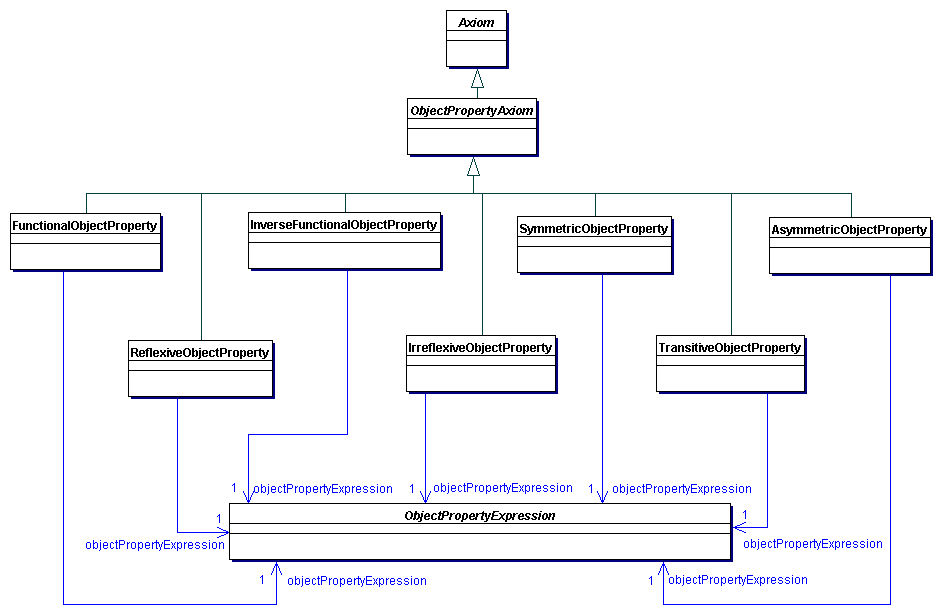
\includegraphics[width=150mm, height=100mm]{Figures/objectpropertyAxiom1.png}
	\caption{Các dạng phát biểu về thuộc tính đối tượng của OWL 2 (phần 2) \label{overflow}}
\end{figure}
Ngoài các dạng phát biểu được nêu, mô tả thuộc tính đối tượng còn có thêm các phát biểu trong hình sau, nhằm quy định tính chất của mô tả thuộc tính đối tượng hay giữa các cá thể được kết nối bằng các thuộc tính đối tượng này, chẳng hạn thuộc tính\textit{ SymmetricObjectProperty} quy định mô tả thuộc tính đối tượng có tính đối xứng - nếu $x$ là bạn $y$ thì $y$ cũng là bạn $x$. 

\paragraph{Functional Object Properties} phát biểu \textit{FunctionalObjectProperty( OPE )} quy định với từng cá thể $x$, chỉ tồn tại nhiều nhất một cá thể $y$ mà $x$ được kết nối với $y$ qua $OPE$. Ví dụ mỗi đối tượng chỉ có tối đa một người cha - \textit{FunctionalObjectProperty( a:hasFather )}. 

\paragraph{Inverse-Functional Object Properties} phát biểu \textit{InverseFunctionalObjectProperty( OPE )} quy định với từng cá thể $x$, chỉ tồn tại nhiều nhất một cá thể $y$ mà $y$ được kết nối qua \textit{OPE} tới $x$ . Ví dụ mỗi tương tự \textit{FunctionalObjectProperty(OPE)}.

\paragraph{Reflexive Object Properties} phát biểu \textit{ReflexiveObjectProperty( OPE )} nói rằng mô tả thuộc tính có tính phản xạ, nghĩa là với từng kết nối bởi \textit{OPE} tới chính nó. Ví dụ: \textit{ReflexiveObjectProperty(a:knows)}, ai cũng biết bản thân họ, với khai báo \textit{ClassAssertion(a:Person a:Peter)} thì có thể suy ra được phát biểu sau \textit{ObjectPropertyAssertion(a:knows a:Peter a:Peter)}.

\paragraph{Irreflexive Object Properties} ngược lại với phát biểu trên  \textit{IrreflexiveObjectProperty( OPE )}, không có cá thể nào tự kết nối với chính nó qua \textit{OPE}. Ví dụ: \textit{IrreflexiveObjectProperty(a:marriedTo)}, không ai cưới chính mình.

\paragraph{Symmetric Object Properties} phát biểu \textit{SymmetricObjectProperty( OPE )} nói rằng \textit{OPE} có tính đối xứng, nếu $x$ nối với $y$ qua \textit{OPE} thì $y$ cũng nối với $x$ bởi \textit{OPE}. Ví dụ: với\textit{ SymmetricObjectProperty( a:friendOf )} và \textit{ObjectPropertyAssertion(a:friend a:Peter a:Bush)} thì chúng ta suy ra được \textit{ObjectPropertyAssertion(a:friend a:Bush a:Peter)}.

\paragraph{Asymmetric Object Properties} phát biểu \textit{AsymmetricObjectProperty( OPE )} nói rằng \textit{OPE} có tính bất đối xứng, nếu $x$ nối với $y$ qua \textit{OPE}, thì $y$ không thể kết nối với $x$ bởi \textit{OPE}. Ví dụ: với \textit{AsymmetricObjectProperty( a:parentOf )}  và \textit{ObjectPropertyAssertion(a:parentOf a:Peter a:Bush)} thì nếu ta thêm thêm phát biểu \textit{ObjectPropertyAssertion(a:parentOf a:Bush a:Peter)} sẽ làm cho ontology mất tính nhất quán (inconsistent).

\paragraph{Transitive Object Properties} phát biểu \textit{TransitiveObjectProperty(OPE)} nói rằng \textit{OPE} có tính bắc cầu, nếu $x$ nối với $y$ bởi \textit{OPE} và $y$ nối với $z$ cũng bằng \textit{OPE} thì $x$ nối với $z$ qua \textit{OPE}. Ví dụ:
\begin{verbatim}
	TransitiveObjectProperty( a:partOf ) 
	ObjectPropertyAssertion( a:partOf a:KhoaMMT a:UIT )
	ObjectPropertyAssertion( a:partOf a:UIT a:VNU )
\end{verbatim}
Giải thích nếu khoa mạng thuộc UIT, UIT thuộc đại học Quốc Gia (VNU), nhờ phát biểu đầu tiến chúng ta $partOf$ có tính chất bắc cầu nên suy ra được khoa mạng thuộc đại học Quốc Gia - \textit{ObjectPropertyAssertion( a:partOf a:KhoaMMT a:VNU)}

% Data Property Axioms
\subsubsection{Các phát biểu về thuộc tính dữ liệu}
\begin{figure}[h]
	\centering
	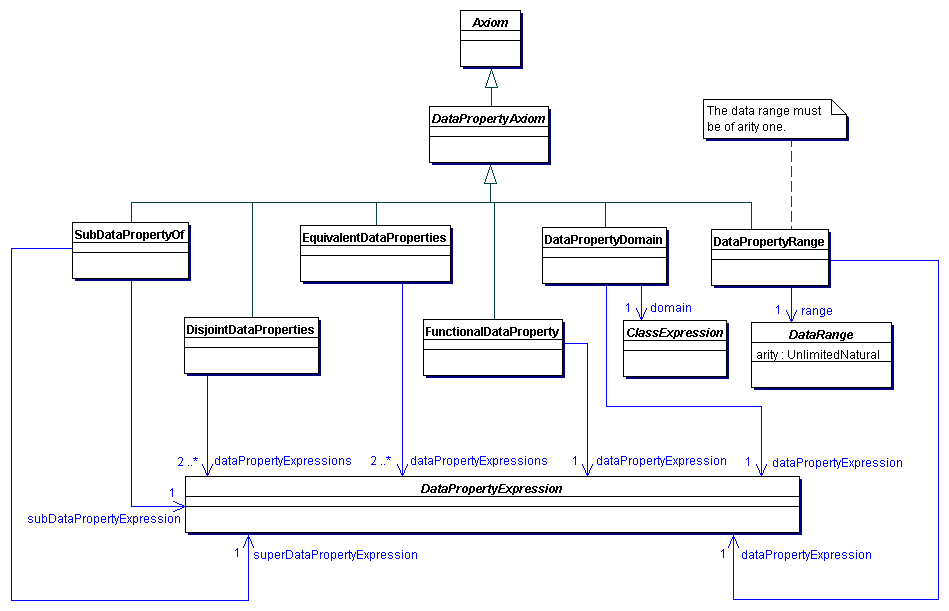
\includegraphics[width=150mm]{Figures/datapropertyAxiom.png}
	\caption{Các dạng phát biểu về thuộc tính dữ liệu của OWL 2 (phần 2) \label{overflow}}
\end{figure}
Cũng giống như mô tả thuộc tính đối tượng, mô tả thuộc tính dữ liệu cũng được cung cấp các phát biểu như \textit{SubDataPropertyOf}, \textit{EquivalentDataProperties}, \textit{DataPropertyDomain}, \textit{DataProperyRange}.

\paragraph{Phát biểu thuộc tính dữ liệu con (Data subproperties)} Phát biểu SubDataPropertyOf( $DPE_{1}$ $DPE_{2}$ ) nói rằng mô tả thuộc tính dữ liệu $DPE_{1}$ là thuộc tính con của mô tả dữ liệu $DPE_{2}$ - có nghĩa nếu một cá thể $x$ được kết nối bởi $DPE_{1}$ tới một trực nghĩa $y$, thì $x$ được kết nối bởi $DPE_{2}$. Ví dụ:
\begin{verbatim}
SubDataPropertyOf( a:hasLastName a:hasName) 
// Họ của một người cũng là tên họ của người đó
DataPropertyAssertion( a:hasLastName a:Peter "Smith" )
// Họ của Peter là "Smith"
\end{verbatim}
\textbf{Giải thích:} vì "có họ" \textbf{(hasLastName)} là thuộc tính con của "có tên" \textit{(hasName)} nên chúng ta ngầm hiểu phát biểu sau mà không cần khai báo tên của Peter là "Smith", tương đương \textit{DataPropertyAssertion(a:hasName a:Peter "Griffin")}

\paragraph{Phát biểu thuộc tính dữ liệu tương đương (Equivalent Data Properties)} Một phát biểu \textit{EquivalentDataProperties( $DPE_{1}$ ... $DPE_{n}$)} nói rằng mỗi mô tả thuộc tính $DPE_{i}$, $1<=i<=n$ đều đồng nghĩa với các tất cả các mô tả thuộc tính còn lại trong phát biểu này phát biểu \textit{EquivalentDataProperties( $DPE_{2}$ $DPE_{1}$ )} cũng tương đương EquivalentDataProperties( $DPE_{1}$ $DPE_{2}$ ). Ví dụ:
\begin{verbatim}
EquivalentDataProperties( a:hasName a:HoTen ) 
// a:hasName tương đượng với a:HoTen trong Tiếng Việt
DataPropertyAssertion( a:hasName a:Peter "Peter Nguyen" )
DataPropertyAssertion( a:HoTen a:Peter "Peter Nguyễn" )
\end{verbatim}
\textbf{Giải thích:} do phát biểu đầu tiên, từ phát biểu thứ 2 ta ngầm hiểu \textit{DataPropertyAssertion( a:hasName a:Peter "Peter Nguyễn" )} tên tiếng Anh "Peter Nguyen" tương đương tên tiếng Viết "Peter Nguyễn" và ngược lại \textit{DataPropertyAssertion( a:HoTen $a:Peter$ "Peter Nguyen") }.

\paragraph{Domain của thuộc tính dữ liệu (Data Property Domain)} Phát biểu \textit{DataPropertyDomain( DPE CE )} nêu rõ domain của thuộc tính dữ liệu là mô tả lớp $CE$ -  nếu một cá thể $x$ được liên kết bởi \textit{DPE} tới vài trực nghĩa nào đó, thì $x$ phải là cá thể thuộc mô tả lớp \textit{CE}.
\begin{verbatim}
DataPropertyDomain( a:hasBankAccount a:Person ) 
// Con người mới có tài khoản ngân hàng
ObjectPropertyAssertion( a:hasBankAccount a:Peter "0002" ) 
// Peter có tài khoản ngân hàng "0002"
\end{verbatim}
\textbf{Giải thích:} không cần thiết phải khai báo Peter là người vì dựa theo chúng ta cũng kết luận được Peter là người từ 2 phát biểu trên, \textit{ClassAssertion(a:Person a:Peter)}.

\paragraph{Miền giá trị của thuộc tính dữ liệu (Data Property Range)} - phát biểu \textit{DataPropertyRange(DPE DR)} nói rằng miền giá trị hợp lệ của mô tả thuộc tính dữ liệu \textit{DPE} là miền dữ liệu \textit{DR} - nếu các cá thể được kết nối bởi \textit{DPE} tới 1 trực nghĩa $x$, thì $x$ trong miền dữ liệu \textit{DR}. Ví dụ:
%Số lượng kết quả đầu ra bắt buộc bằng 1, tức không tồn tại $x \equiv y \equiv z$, với $y \not\equiv z$ và $y, z \in DR$.
\begin{verbatim}
DataPropertyRange( a:hasName xsd:string )
DataPropertyAssertion( a:hasName a:Peter "Peter Nguyen" )
\end{verbatim}
Nếu khai báo sau sẽ làm cho ontology bị thiếu nhất quán (inconsistent):
\begin{verbatim}
DataPropertyAssertion( a:hasName a:Peter "42"^^xsd:integer)
\end{verbatim}

\paragraph{Functional Data Properties} - phát biểu \textit{FunctionalDataProperty(DPE)} nói rằng với mỗi $x$, chỉ có nhiều nhất một trực nghĩa $y$ mà $x$ được gán cho bởi \textit{DPE}. Ví dụ:
\begin{verbatim}
FunctionalDataProperty( a:hasAge )
// Mọi đối tượng chỉ có tối đa một số tuổi
DataPropertyAssertion( a:hasAge a:Steve "17"^^xsd:integer )
\end{verbatim}
Các phát biểu trên sẽ bị thiếu nhất quán nếu chúng ta thêm vào phát biểu sau 
\begin{verbatim}
DataPropertyAssertion( a:hasAge a:Steve "15"^^xsd:integer)
\end{verbatim}

%% Assertions
\subsubsection{Các phát biểu về cá thể (Assertions)} 
\begin{figure}[H]
	\centering
	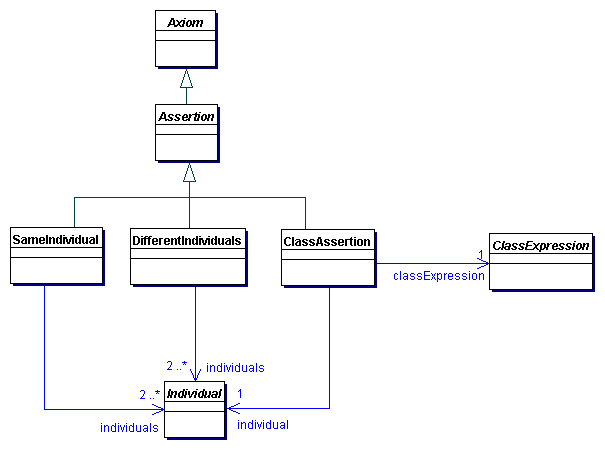
\includegraphics[width=120mm]{Figures/abox1.png}
	\caption{Các phát biểu gán lớp cho cá thể và cá thể giống nhau/khác nhau trong OWL 2 \label{overflow}}
\end{figure}

\begin{figure}[ht!]
	\centering
	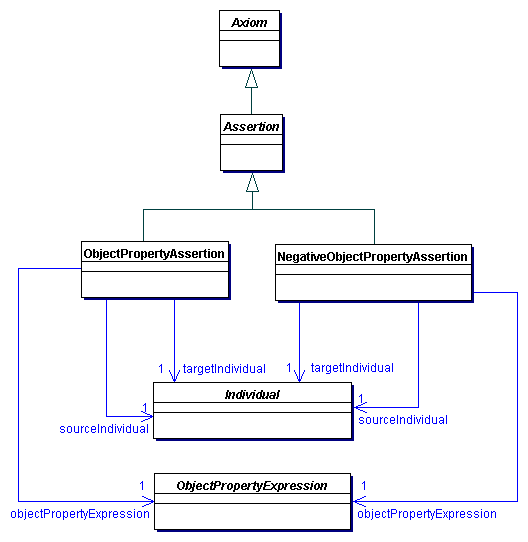
\includegraphics[width=120mm,height=110mm]{Figures/abox2.png}
	\caption{Các phát biểu về thuộc tính đối trượng của cá thể trong OWL 2 \label{overflow}}
\end{figure}

\begin{figure}[hb!]
	\centering
	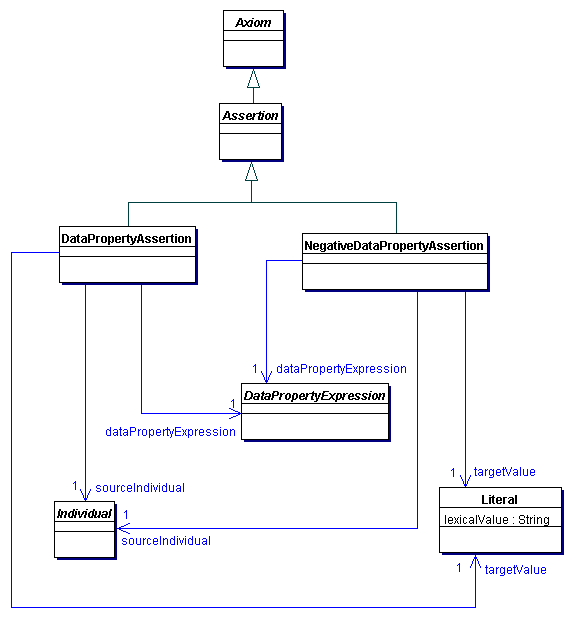
\includegraphics[width=120mm,height=110mm]{Figures/abox3.png}
	\caption{Các phát biểu về thuộc tính dữ liệu của cá thể trong OWL 2 \label{overflow}}
\end{figure}
Các phát biểu về cá thể thường được gọi là \textit{facts}. Để rõ hơn, các loại assertions khác nhau được thể hiện trong các hình sau.

\begin{description}
\item[SameIndividual] - khẳng định sự tương đồng của các cá thể trong phát biểu.

\item[DifferentIndividuals] - khẳng định sự khác nhau của các cá thể trong phát biểu.

\item[ClassAssertion] - khẳng định một cá thể thuộc một mô tả lớp/ lớp cụ thể trong phát biểu.

\item[ObjectPropertyAssertion] - khẳng định mối quan hệ từ một cá thể tới một cá thể nào đó bởi một mô tả thuộc tính đối tượng.

\item[NegativeObjectPropertyAssertion] - phủ định mối quan hệ từ một cá thể tới một cá thể khác bởi một mô tả thuộc tinh đối tượng.

\item[DataPropertyAssertion] - khẳng định mối quan hệ từ một cá thể tới một trực nghĩa bởi một mô tả thuộc tính dữ liệu.

\item[NegativeDataPropertyAssertion] - phủ định mối quan hệ từ một cá thể tới một trực nghĩa bởi một mô tả thuộc tính dữ liệu.
\end{description}

\paragraph{Kết luận} - Trên đây, chúng em đã trình bày những thành phần chính của OWL2 cũng như cách sử dụng của chúng trong quá trình suy luận (reasoning) nhằm tìm ra hàm ý, phát hiện thông tin ẩn chứa trong ý nghĩa của những phát biểu đã khai báo, với mục đích cuối cùng là phục vụ cho quá trình phân loại tự động. Vì độ dài luận văn hạn chế, nên có một số thành phần của OWL 2 chưa được nêu ra ở đây như \textbf{Datatype Definitions}, \textbf{Keys}, \textbf{Annotations}, \textbf{Datatype Maps} xin mời quý thầy cô và các bạn đọc tham khảo thêm ở \cite{owl2spec}. Chương tiếp theo chúng em xin được giới thiệu về Semantic Web Rule Language, một ngôn ngữ điều luật (rule language) có tác dụng trong việc tăng tính quyết định cho ontology, đồng thời chúng em cũng muốn nêu ra các nguyên nhân dẫn đến tính thiếu nhất quán trong ontology (inconsistency), và các giải pháp nhằm làm giảm các nguyên nhân đó.